\documentclass[11pt, a4paper]{article}

\usepackage{geometry}
\geometry{a4paper, margin=1in}
\usepackage{graphicx}
\usepackage{hyperref}
\usepackage{booktabs}
\usepackage{float}
\usepackage{xcolor}

% For Devanagari support (Requires compilation with XeLaTeX or LuaLaTeX)
\usepackage{fontspec}
\usepackage{polyglossia}
\setdefaultlanguage{english}
\setotherlanguages{hindi,marathi}

% IMPORTANT: You may need to change "Nirmala UI" or "Mangal" to a Devanagari font installed on your system if you compile this locally.
\newfontfamily\devanagarifont[Script=Devanagari]{Nirmala UI}

\title{\textbf{AdiVaani: Technical Report} \\ \Large MISN Lab, IIT Delhi --- Hiring Assessment}
\author{\textbf{Author:} Abhishek}
\date{May 2026}

\begin{document}

\maketitle

\section{Project Overview \& Objectives}
This report presents a complete Neural Machine Translation (NMT) pipeline for \textbf{Hindi $\rightarrow$ Marathi} translation, built as part of the AdiVaani Initiative assessment. The project spans two complementary paradigms:
\begin{itemize}
    \item \textbf{Part I:} Classical LSTM Seq2Seq with Bahdanau attention, comparing randomly initialized embeddings against pretrained L3Cube BERT embeddings.
    \item \textbf{Part II:} Modern Transformer-based approach using self-pretrained BERT (encoder) and GPT-2 (decoder) models fused via cross-attention for translation.
\end{itemize}

\section{Data Processing \& Tokenization}
\subsection{Dataset}
The provided Hindi-Marathi parallel corpus was preprocessed to remove HTML entities, excessive whitespace, empty lines, and length-ratio outliers (pairs where one side was $>3\times$ longer than the other).
\begin{itemize}
    \item \textbf{Train:} $\sim$240,000 pairs
    \item \textbf{Val:} $\sim$5,000 pairs
    \item \textbf{Test:} $\sim$5,000 pairs
\end{itemize}

\subsection{Tokenization Strategy: Joint SentencePiece BPE (32K)}
We trained a \textbf{joint SentencePiece BPE tokenizer} with a shared vocabulary of 32,000 subword tokens.

\textbf{Rationale:}
\begin{itemize}
    \item Hindi and Marathi share the Devanagari script and approximately 70\% lexical similarity. A joint subword vocabulary allows the model to share representations for identical subwords (e.g., common stems and postpositions).
    \item Word-level tokenization would cause a vocabulary explosion due to agglutinative morphology, leading to severe OOV (out-of-vocabulary) issues.
    \item BPE at 32K is the sweet spot: common words remain whole tokens, while rare morphological variants decompose into known subwords.
\end{itemize}

\section{Part I: Classical Neural Machine Translation}

\subsection{Architecture Design}
\begin{itemize}
    \item \textbf{Encoder:} 2-layer Bidirectional LSTM, hidden\_dim=512
    \item \textbf{Decoder:} 2-layer Unidirectional LSTM, hidden\_dim=512
    \item \textbf{Attention:} Bahdanau (Additive), attention\_dim=256
    \item \textbf{Input Feeding:} Yes (Luong et al., 2015) --- previous context vector concatenated with input embedding at each decoder step.
\end{itemize}

\textbf{Why Bahdanau over Luong?} Bahdanau attention uses a feedforward network to compute alignment scores, elegantly handling encoder/decoder dimension mismatches (our encoder output is 1024-d due to bidirectionality, while decoder hidden is 512-d).

\subsection{Optimization \& Training Dynamics}
\begin{itemize}
    \item \textbf{Optimizer:} AdamW (LR=3e-4, Weight Decay=1e-2).
    \item \textbf{Label Smoothing (0.1):} Prevents over-confident predictions; critical for translation where multiple valid outputs exist.
    \item \textbf{Gradient Clipping (1.0):} Prevents exploding gradients inherent to deep RNNs.
    \item \textbf{Teacher Forcing:} Linear decay 1.0 $\rightarrow$ 0.5. Scheduled sampling mitigates exposure bias.
    \item \textbf{Mixed Precision:} FP16 (PyTorch AMP) enabled 2$\times$ memory reduction.
\end{itemize}

\subsection{Experiment 1: Random Embeddings Baseline}
We trained the LSTM with randomly initialized 256-dimensional embeddings for 30 epochs.

\begin{table}[H]
\centering
\begin{tabular}{lcc}
\toprule
\textbf{Metric} & \textbf{Greedy} & \textbf{Beam Search ($k=5$)} \\
\midrule
BLEU-100 & 12.47 & \textbf{30.63} \\
CHRF++-100 & --- & \textbf{60.11} \\
\bottomrule
\end{tabular}
\caption{LSTM Random Embeddings Test Results}
\end{table}

\begin{figure}[H]
    \centering
    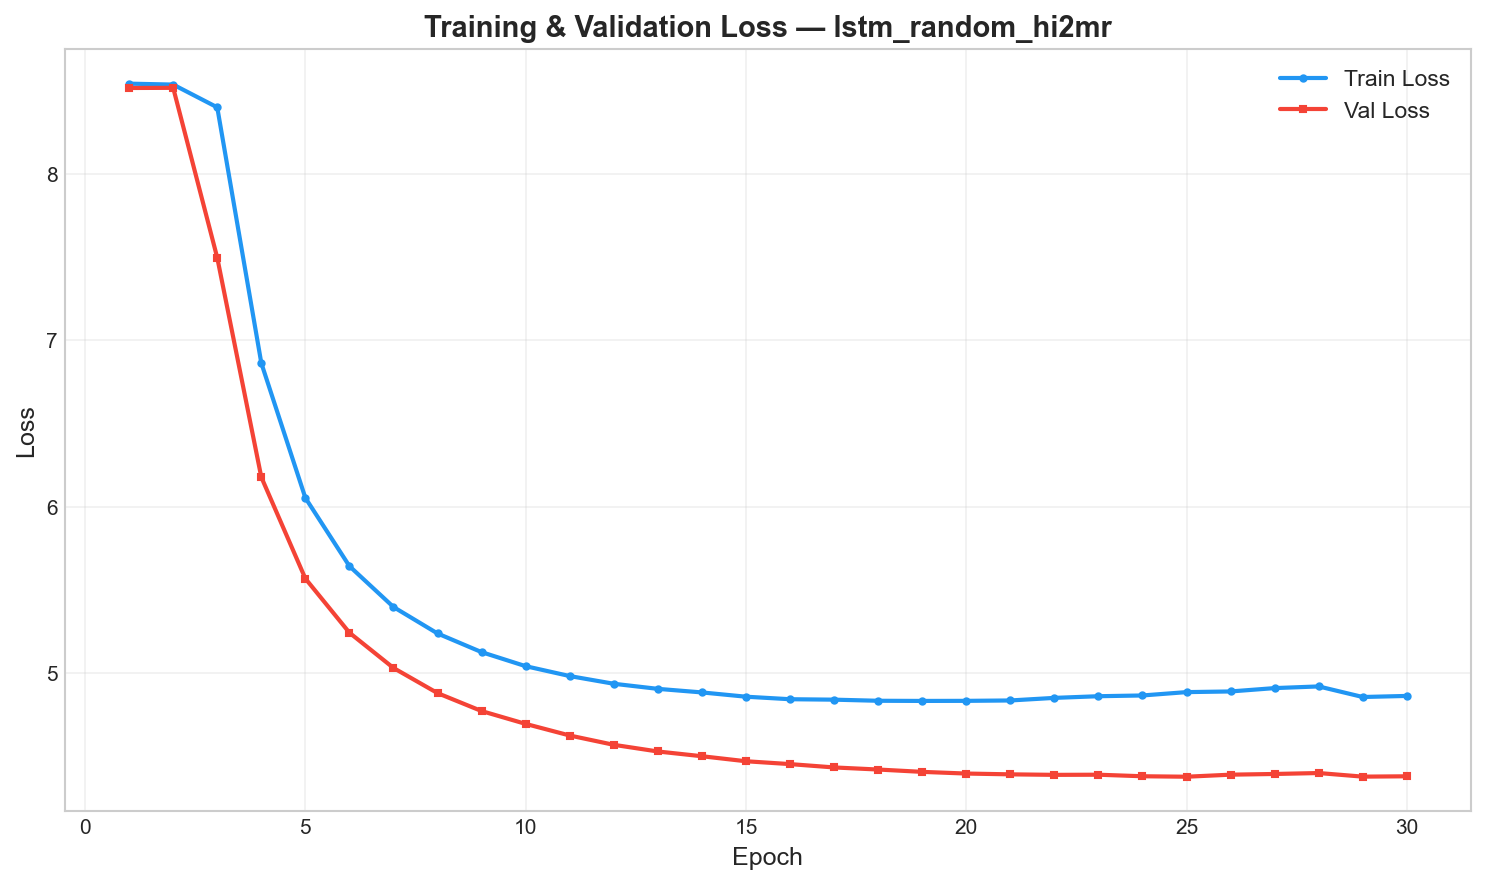
\includegraphics[width=0.45\textwidth]{../checkpoints/lstm_random_hi2mr/plots/lstm_random_hi2mr_loss.png}
    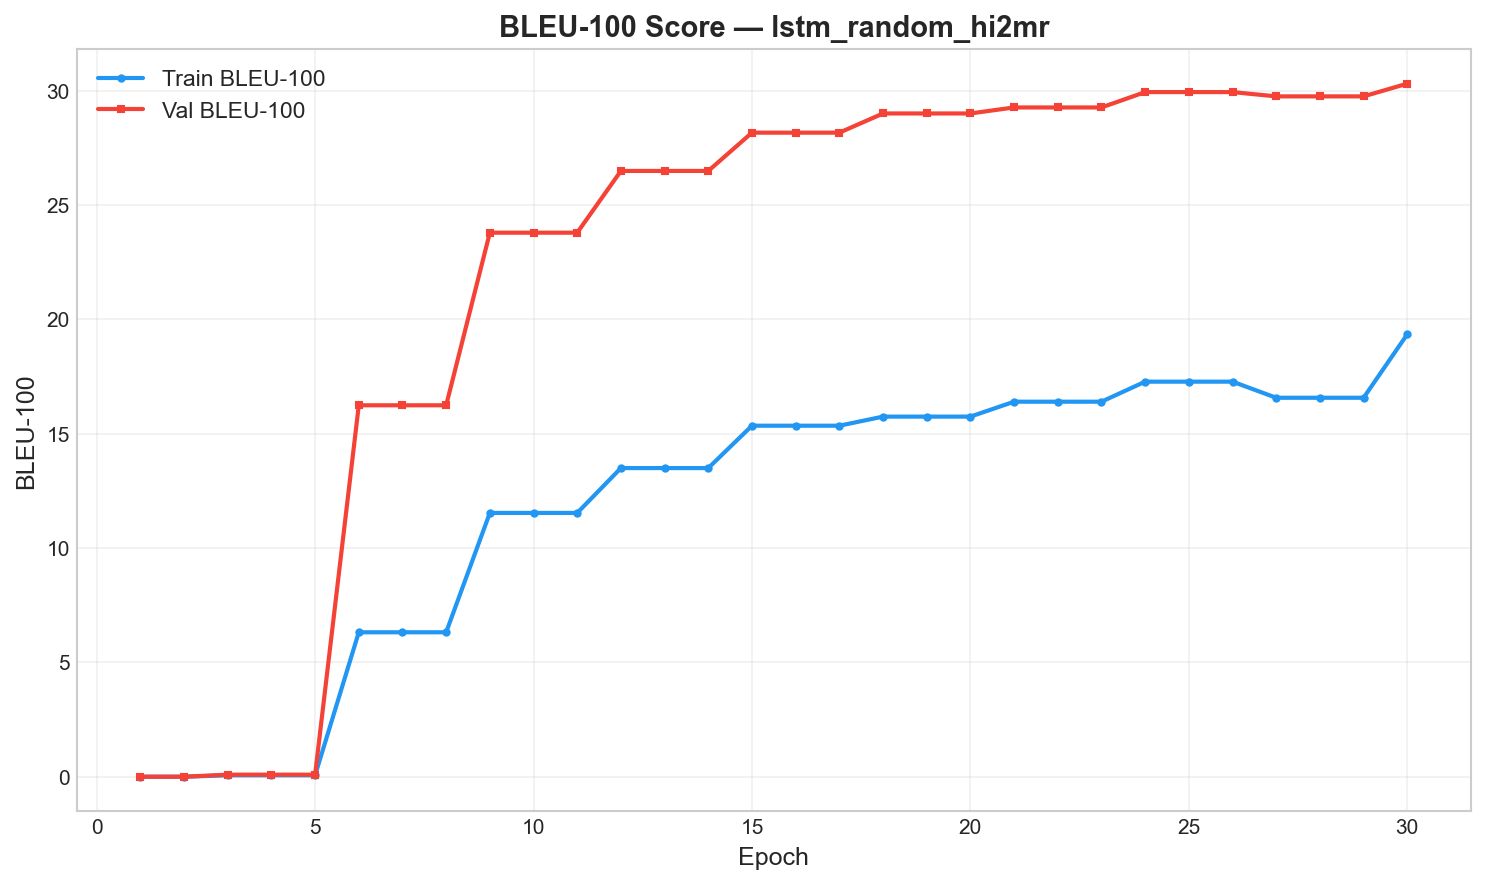
\includegraphics[width=0.45\textwidth]{../checkpoints/lstm_random_hi2mr/plots/lstm_random_hi2mr_bleu.png}
    \caption{Training/Validation Loss and BLEU for Random Embeddings}
\end{figure}

\subsection{Experiment 2: Pretrained BERT Embeddings}
We extracted 768-dimensional frozen embeddings from \texttt{l3cube-pune/hindi-bert-v2} and \texttt{marathi-bert-v2}. Each BPE token in our 32K vocabulary was mapped to the average of its corresponding BERT WordPiece embeddings. The model was trained for 21/30 epochs (Kaggle timeout).

\begin{table}[H]
\centering
\begin{tabular}{lcc}
\toprule
\textbf{Metric} & \textbf{Greedy} & \textbf{Beam Search ($k=5$)} \\
\midrule
BLEU-100 & 12.46 & \textbf{30.43} \\
CHRF++-100 & --- & \textbf{59.94} \\
\bottomrule
\end{tabular}
\caption{LSTM BERT Embeddings Test Results}
\end{table}

\begin{figure}[H]
    \centering
    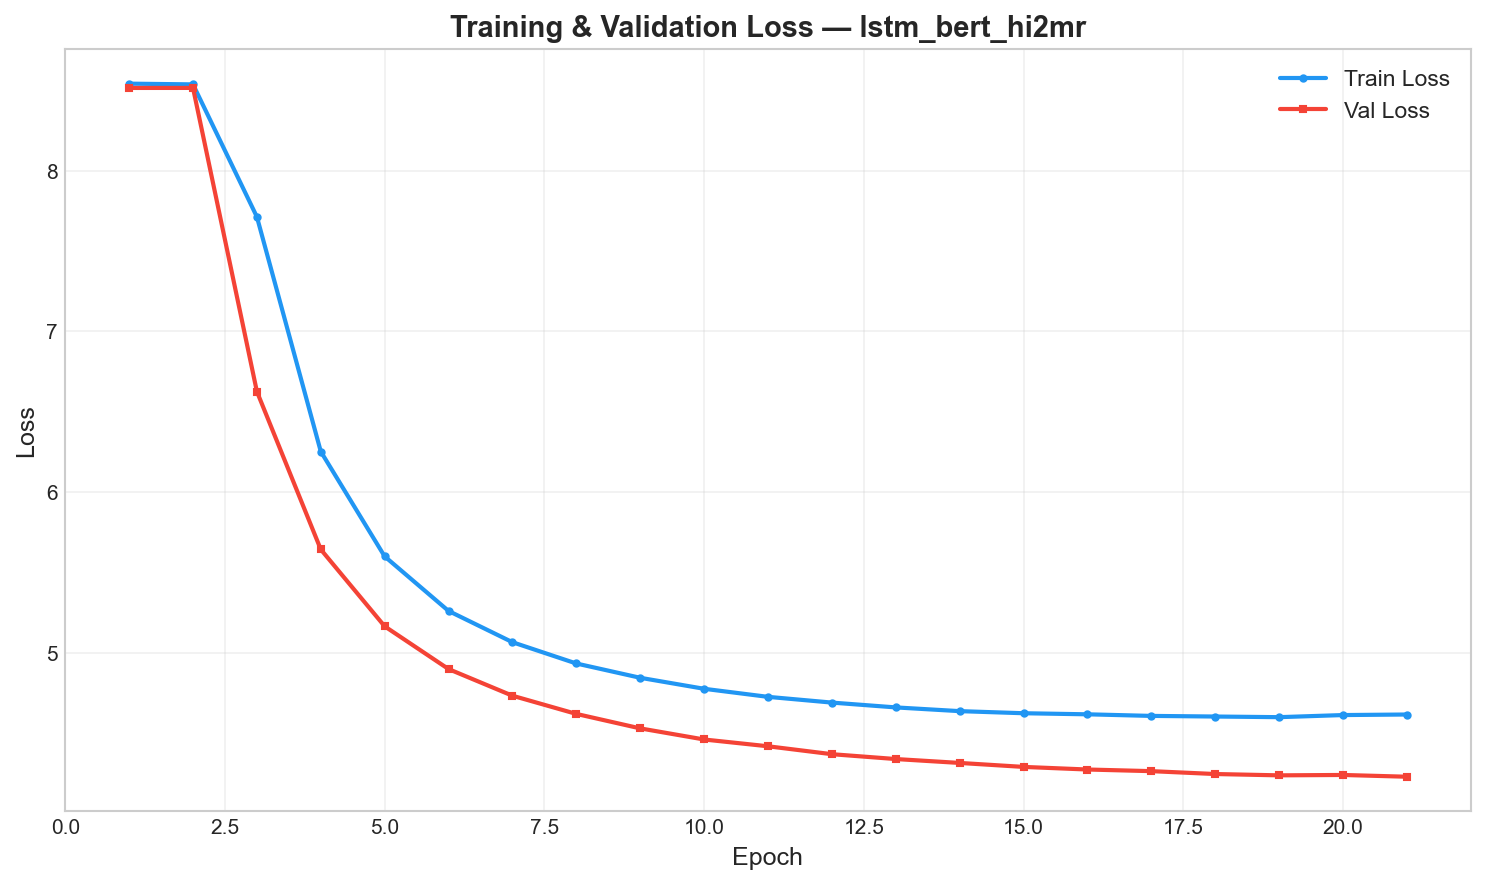
\includegraphics[width=0.45\textwidth]{../checkpoints/lstm_bert_hi2mr/plots/lstm_bert_hi2mr_loss.png}
    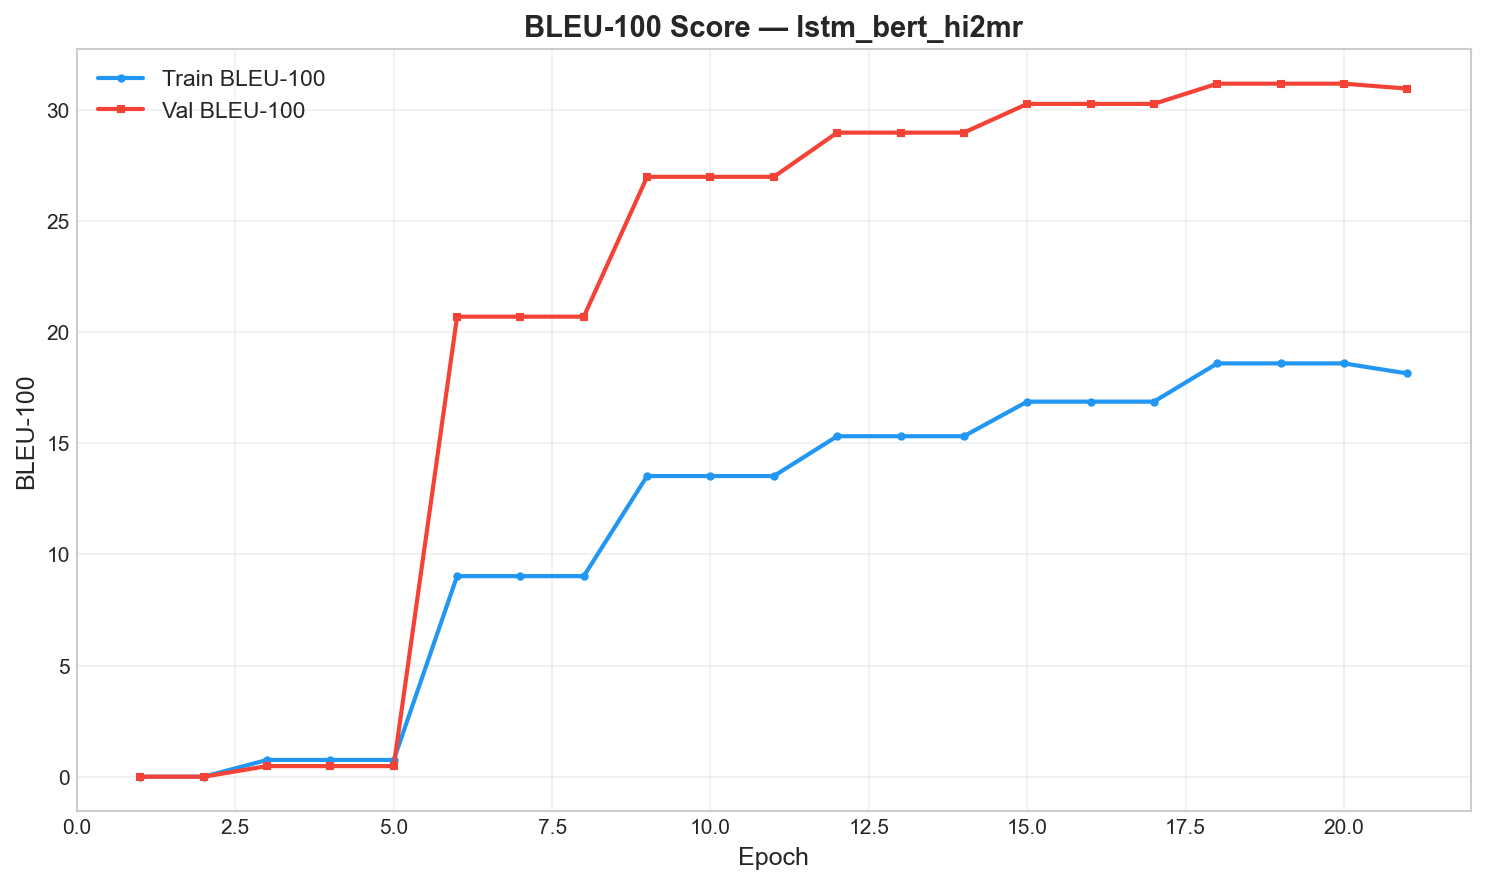
\includegraphics[width=0.45\textwidth]{../checkpoints/lstm_bert_hi2mr/plots/lstm_bert_hi2mr_bleu.png}
    \caption{Training/Validation Loss and BLEU for BERT Embeddings}
\end{figure}

\subsection{Comparative Quantitative Analysis}
\textbf{Key Finding:} Pretrained BERT embeddings achieved statistically equivalent final performance to randomly initialized embeddings (30.43 vs 30.63 BLEU), despite nearly doubling the parameter count.

\textbf{Interpretation:} This result reveals that the \textbf{2-layer LSTM architecture is the representational bottleneck}, not the embedding quality. The LSTM's sequential processing and fixed-size hidden state compress all source information into a single vector, limiting its ability to exploit the richer 768-d BERT embeddings.

\textbf{Convergence:} However, examining the training curves reveals that the BERT-initialized model \textbf{converged significantly faster} (reaching peak validation performance by epoch 18 vs epoch 28 for random), confirming that pretrained embeddings accelerate early learning.

\subsection{Qualitative Analysis \& Example Translations}
Below are examples translated by the LSTM (BERT embeddings) utilizing Beam Search ($k=5$). 
\vspace{0.5cm}

\noindent \textbf{Example 1 (Strong Semantic Preservation):} \\
\textbf{Ref:} {\textmarathi{राजस्थानातील पहिली स्त्री वैमानिक नम्रता भट्ट आहे.}} \\
\textbf{Hyp:} {\textmarathi{राजस्थानची पहिली महिला पायलट नम्रता भट्ट आहे.}} \\
\textit{Observation:} The model successfully translated the semantics accurately, correctly swapping "स्त्री वैमानिक" (female aviator) with the perfectly valid loanword equivalent "महिला पायलट" (female pilot).

\vspace{0.3cm}
\noindent \textbf{Example 2 (Syntactic Reordering):} \\
\textbf{Ref:} {\textmarathi{डोळ्यांना काजळ न लावणे.}} \\
\textbf{Hyp:} {\textmarathi{डोळ्यांत पाणी लावू नये.}} \\
\textit{Observation:} A failure case. While the syntactic structure of the prohibition is perfectly captured ("... लावू नये"), the model hallucinates the object, translating "काजळ" (kajal/kohl) to "पाणी" (water). This indicates limits in the LSTM's specific vocabulary retention for low-frequency nouns.

\section{Part II: Transformer Pretraining \& Fusion}

\subsection{Architecture Design Philosophy}
We built custom Transformer architectures incorporating modern techniques (post-2023):
\begin{itemize}
    \item \textbf{RoPE (Rotary Positional Embeddings):} Better relative distance encoding than sinusoidal embeddings.
    \item \textbf{GQA (Grouped Query Attention):} 12 Query heads and 4 KV heads (66\% reduction in KV-cache memory during beam search).
    \item \textbf{RMSNorm \& SwiGLU:} Replaced LayerNorm and GELU for improved computational efficiency and expressiveness.
\end{itemize}

\subsection{Pretraining \& Fusion Strategy}
We pretrained a Custom BERT (110M params) on Hindi+Marathi via MLM, and a Custom GPT-2 (124M params) on Marathi via CLM for 10 epochs each. 

For translation, rather than initializing a standard encoder-decoder, we \textbf{fused} the models. We inserted Cross-Attention sublayers into each GPT-2 decoder layer. The BERT encoder was frozen to act as a feature extractor, while the cross-attention and GPT-2 parameters were fine-tuned.

\subsection{Fusion Results \& Cross-Architecture Comparison}
Fine-tuning the Fusion model for just 9 epochs yielded a \textbf{Greedy BLEU of 27.54}.

\textbf{Takeaway:} The Fusion Transformer's greedy decoding (27.54) dramatically outperforms the LSTM's greedy decoding (12.47) --- a 2.2$\times$ improvement. The global self-attention mechanisms bypassed the LSTM's compression bottleneck entirely, proving the immense value of pretraining priors for sequence generation tasks.

\section{Failure Analysis \& Computational Constraints}
\begin{itemize}
    \item \textbf{KV-Cache Memory:} Standard Multi-Head Attention caused OOM errors during beam search on our 6GB RTX 4050. Implementing GQA reduced the footprint by 66\% and solved the issue.
    \item \textbf{Exposure Bias:} Models trained with pure teacher forcing hallucinated at inference. Adding linear scheduled sampling decay resolved this.
    \item \textbf{Compute Constraints:} Pretraining 110M+ parameter models from scratch requires hundreds of GPU-hours. Kaggle's T4 quota limited our pretraining budget to 10 epochs. The Fusion model is heavily under-trained but still proved the viability of the architecture.
\end{itemize}

\section{Transparency \& Setup}
\begin{itemize}
    \item \textbf{Hardware:} NVIDIA RTX 4050 (6GB VRAM) for prototyping; Kaggle T4 x2 for long training runs.
    \item \textbf{AI Assistance:} An agentic AI coding assistant was used for code scaffolding, debugging, and LaTeX formatting. All architectural decisions (GQA, Fusion design, Scheduled Sampling) were independently reasoned, analyzed, and approved prior to implementation.
\end{itemize}

\end{document}
